\documentclass[12pt,a4paper,oneside]{article}

% ========== 页面与字体 ==========
\usepackage{geometry}
\geometry{left=2.5cm,right=2.5cm,top=3cm,bottom=3cm}

% ========== 中文支持 ==========
\usepackage{xeCJK}
\xeCJKsetup{
    CJKspace=true,
    CJKmath=true,
    xCJKecglue={}
}
\setCJKmainfont{SimSun}
\setCJKsansfont{SimHei}
\setCJKmonofont{FangSong}

% ========== 数学宏包 ==========
\usepackage{amsmath}
\usepackage{amssymb}
\usepackage{amsfonts}
\usepackage{mathtools}
\numberwithin{equation}{section}
\DeclareMathOperator{\sgn}{sgn}
\DeclareMathOperator{\diag}{diag}

% ========== 图形与表格 ==========
\usepackage{graphicx}
\usepackage{float}
\usepackage{subcaption}
\usepackage{booktabs}
\usepackage{multirow}
\usepackage{longtable}
\usepackage{array}
\usepackage{diagbox}
\usepackage{ccicons}

% ========== 代码高亮 ==========
\usepackage{listings}
\lstset{
    language=Matlab,
    basicstyle=\ttfamily\small,
    keywordstyle=\color{blue}\bfseries,
    commentstyle=\color{green!60!black},
    stringstyle=\color{red!60!black},
    numbers=left,
    numberstyle=\tiny\color{gray},
    breaklines=true,
    frame=single,
    backgroundcolor=\color{blue!5},
    basicstyle=\fontsize{9}{11}\selectfont\ttfamily
}

% ========== 标题格式 ==========
\usepackage{titlesec}
\titleformat{\section}{\bfseries\Large\raggedright}{\thesection}{1em}{}
\titleformat{\subsection}{\bfseries\large\raggedright}{\thesubsection}{1em}{}
\titleformat{\subsubsection}{\bfseries\normalsize\raggedright}{\thesubsubsection}{1em}{}

% ========== 页眉页脚 ==========
\usepackage{fancyhdr}
\pagestyle{fancy}
\fancyhf{}
\fancyhead[L]{\setCJKfont\CJKfamily{hei}\small 前馈控制实验指导书}
\fancyhead[R]{\thepage}
\fancyfoot[C]{\thepage}
\setlength{\headheight}{14pt}

% ========== 十字线 ==========
\usepackage{ulem}
\usepackage{enumerate}

% ========== 超链接 ==========
\usepackage[colorlinks=true,linkcolor=blue,citecolor=blue,urlcolor=blue]{hyperref}

% ========== 首行缩进 ==========
\usepackage{indentfirst}
\setlength{\parindent}{2em}
\setlength{\parskip}{0.5em}

% ========== 页脚 ==========
\usepackage{lastpage}

% ========== 自定义命令 ==========
\newcommand{\ee}[1]{\mathrm{e}^{#1}}
\newcommand{\dd}[1]{\mathrm{d}{#1}}
\newcommand{\bb}[1]{\mathbf{#1}}
\newcommand{\norm}[1]{\left\lVert#1\right\rVert}
\newtheorem{assumption}{假设}
\newtheorem{property}{性质}
\newtheorem{conclusion}{结论}

% ========== 标题页 ==========
\title{\textbf{\Huge 机械臂前馈控制实验指导书}\\[2em]
    \large XB4 六自由度机械臂的计算力矩前馈控制}
\author{\CJKfamily{hei} 智能机器人技术课程}
\date{\CJKfamily{kai}\large \today}

\begin{document}

% ========== 封面 ==========
\begin{titlepage}
    \centering
    \vspace*{2cm}
    {\Huge\CJKfamily{hei}\bfseries 机械臂前馈控制实验指导书}\\[2cm]
    {\LARGE XB4 六自由度机械臂\\计算力矩前馈控制}\\[3cm]
    {\Large\CJKfamily{kai} 智能机器人技术课程实验}\\[2cm]
    {\Large 2026 年 4 月}\\[4cm]
    \thispagestyle{empty}
\end{titlepage}
\thispagestyle{empty}
\newpage

% ========== 目录 ==========
\pagenumbering{Roman}
\tableofcontents
\newpage

% ========== 正文 ==========
\pagenumbering{arabic}
\pagestyle{fancy}

% ==================== 第一章：引言 ====================
\section{引言}

\subsection{研究背景}

机械臂作为工业自动化和智能制造中的核心装备，其运动控制精度直接影响生产效率和产品质量。
在机械臂控制中，关节空间的轨迹跟踪是一个基础而重要的问题~\cite{spong2005robot}。
由于机械臂具有强耦合、非线性、多输入多输出等特性，传统的独立关节 PID 控制
在高速、高精度要求的场景下往往难以满足需求。

\textbf{前馈控制（Feedforward Control）}是一种基于被控对象模型的先进控制策略，
其核心思想是利用系统模型提前计算为实现期望运动所需的控制输入，
再叠加反馈控制来补偿模型误差和外部扰动。
对于机械臂系统，前馈控制通常以\textbf{计算力矩法（Computed Torque Method）}的形式实现，
也被称为\textbf{逆动力学前馈}。

本实验以 XB4 六自由度串联机械臂为对象，
在 MATLAB/Simulink 仿真平台上实现前馈控制与 PID 控制的对比实验，
通过轨迹跟踪误差和关节力矩的对比，直观展示前馈控制对机械臂控制性能的提升。

\subsection{实验目标}

本实验的主要目标包括：

\begin{enumerate}
    \item 理解机械臂动力学建模的基本原理，掌握 D-H 参数法和 Newton-Euler 动力学算法；
    \item 理解前馈控制的基本思想，掌握计算力矩前馈控制律的推导过程；
    \item 在 MATLAB/Simulink 平台上实现 XB4 机械臂的前馈控制系统；
    \item 通过对比实验，分析前馈控制对轨迹跟踪精度和控制性能的改善效果；
    \item 观察不同运动频率下前馈控制效果的差异，理解前馈项在高速运动中的重要性。
\end{enumerate}

\subsection{实验设备}

\begin{itemize}
    \item 计算机（安装 MATLAB R2020b 及以上版本）
    \item MATLAB/Simulink 仿真平台
    \item XB4 机械臂模型参数文件（\texttt{set\_mode\_parameter.m}）
    \item Simulink 仿真模型（\texttt{sia003A.slx}）
\end{itemize}

% ==================== 第二章：理论基础 ====================
\section{理论基础}

\subsection{机械臂运动学基础}

\subsubsection{D-H 参数法}

机械臂运动学研究关节空间到任务空间的映射关系。
\textbf{Denavit-Hartenberg (D-H) 参数法}是建立串联机械臂运动学模型的标准方法，
通过在每个关节处建立坐标系，利用四个参数描述相邻连杆之间的相对位姿。

对于一个具有 $n$ 个转动关节的机械臂，连杆 $i$ 的 D-H 参数包括：

\begin{table}[H]
    \centering
    \caption{D-H 参数定义}
    \begin{tabular}{ccp{7cm}}
        \toprule
        \textbf{参数} & \textbf{符号} & \textbf{物理意义} \\
        \midrule
        关节转角 & $\theta_i$ & 绕 $z_{i-1}$ 轴从 $x_{i-1}$ 到 $x_i$ 的角度 \\
        连杆偏距 & $d_i$ & 沿 $z_{i-1}$ 轴从 $x_{i-1}$ 到 $x_i$ 的距离 \\
        连杆长度 & $a_i$ & 沿 $x_i$ 轴从 $z_{i-1}$ 到 $z_i$ 的距离 \\
        连杆扭角 & $\alpha_i$ & 绕 $x_i$ 轴从 $z_{i-1}$ 到 $z_i$ 的角度 \\
        \bottomrule
    \end{tabular}
\end{table}

相邻连杆坐标系 $\{i-1\}$ 到 $\{i\}$ 的齐次变换矩阵为：

\begin{equation}
    {}^{i-1}T_i = \begin{bmatrix}
        \cos\theta_i & -\sin\theta_i\cos\alpha_i &  \sin\theta_i\sin\alpha_i & a_i\cos\theta_i \\
        \sin\theta_i &  \cos\theta_i\cos\alpha_i & -\cos\theta_i\sin\alpha_i & a_i\sin\theta_i \\
        0            &  \sin\alpha_i              &  \cos\alpha_i              & d_i             \\
        0            &  0                         &  0                         & 1
    \end{bmatrix}
    \label{eq:dh_transform}
\end{equation}

通过依次连乘各连杆的变换矩阵，可得到末端执行器相对于基座的位置和姿态：

\begin{equation}
    {}^{0}T_n = {}^{0}T_1 \cdot {}^{1}T_2 \cdot \cdots \cdot {}^{n-1}T_n
    \label{eq:forward_kinematics}
\end{equation}

\subsubsection{XB4 机械臂的 D-H 参数}

XB4 机械臂具有 6 个转动关节，其 D-H 参数如下表所示：

\begin{table}[H]
    \centering
    \caption{XB4 机械臂 D-H 参数表}
    \begin{tabular}{cccccc}
        \toprule
        \textbf{关节 $i$} & $\theta_i$ & $d_i$ (m) & $a_i$ (m) & $\alpha_i$ & \textbf{关节类型} \\
        \midrule
        1 & $q_1$        & 0.342 & 0.040 & $0$        & 转动 \\
        2 & $q_2 - \pi/2$ & $0$   & 0.275 & $-\pi/2$   & 转动 \\
        3 & $q_3$        & $0$   & 0.025 & $0$        & 转动 \\
        4 & $q_4$        & 0.280 & $0$   & $-\pi/2$   & 转动 \\
        5 & $q_5$        & $0$   & $0$   & $\pi/2$    & 转动 \\
        6 & $q_6$        & 0.073 & $0$   & $-\pi/2$   & 转动 \\
        \bottomrule
    \end{tabular}
\end{table}

\subsection{机械臂动力学基础}

机械臂动力学描述关节力矩与关节运动（位置、速度、加速度）之间的数学关系，
是前馈控制的核心。本节介绍两种主流的动力学建模方法。

\subsubsection{拉格朗日方程}

对于 $n$ 自由度机械臂，其动力学方程可以统一写成：

\begin{equation}
    \bb{M}(\bb{q})\ddot{\bb{q}} + \bb{C}(\bb{q},\dot{\bb{q}})\dot{\bb{q}} + \bb{G}(\bb{q}) = \bb{\tau}
    \label{eq:robot_dynamics}
\end{equation}

其中：

\begin{itemize}
    \item $\bb{q} \in \mathbb{R}^n$：关节位置向量
    \item $\bb{M}(\bb{q}) \in \mathbb{R}^{n \times n}$：惯性矩阵（对称正定）
    \item $\bb{C}(\bb{q},\dot{\bb{q}}) \in \mathbb{R}^n$：哥氏力和离心力项
    \item $\bb{G}(\bb{q}) \in \mathbb{R}^n$：重力项
    \item $\bb{\tau} \in \mathbb{R}^n$：关节驱动力矩
\end{itemize}

式~\eqref{eq:robot_dynamics} 的物理含义：
\begin{itemize}
    \item $\bb{M}(\bb{q})\ddot{\bb{q}}$：克服惯性所需的力矩
    \item $\bb{C}(\bb{q},\dot{\bb{q}})\dot{\bb{q}}$：克服哥氏力和离心力的力矩
    \item $\bb{G}(\bb{q})$：克服重力的力矩
    \item $\bb{\tau}$：电机提供的总驱动力矩
\end{itemize}

惯性矩阵 $\bb{M}(\bb{q})$ 是理解前馈控制的关键。对于非线性系统~\eqref{eq:robot_dynamics}，
若能精确知道 $\bb{M}$、$\bb{C}$、$\bb{G}$，则可以通过非线性控制律将其线性化。

\subsubsection{Newton-Euler 算法}

直接使用拉格朗日方程计算动力学需要求导大量三角函数，计算量大。
\textbf{Newton-Euler (NE) 算法}是一种递推算法，计算效率更高，
被广泛应用于实时控制中的逆动力学计算。

NE 算法分为\textbf{正向递推}和\textbf{反向递推}两个阶段：

\textbf{第一阶段：正向递推（计算各连杆的速度和加速度）}

从基座到末端执行器依次计算各连杆的角速度、角加速度和线加速度：

\begin{align}
    {}^{i}\omega_i &= {}^{i-1}R_i^{\top}\left({}^{i-1}\omega_{i-1} + \dot{q}_i \hat{z}\right) \\
    {}^{i}\dot{\omega}_i &= {}^{i-1}R_i^{\top}\left[{}^{i-1}\dot{\omega}_{i-1} + \dot{q}_i \hat{z} + {}^{i-1}\omega_{i-1} \times \dot{q}_i \hat{z}\right] \\
    {}^{i}\dot{v}_i &= {}^{i-1}R_i^{\top}\left\{{}^{i-1}\dot{\omega}_{i-1} \times {}^{i-1}p_i + {}^{i-1}\omega_{i-1} \times \left({}^{i-1}\omega_{i-1} \times {}^{i-1}p_i\right) + {}^{i-1}\dot{v}_{i-1}\right\} \\
    {}^{i}\dot{v}_{c,i} &= {}^{i}\dot{\omega}_i \times {}^{i}r_{c,i} + {}^{i}\omega_i \times \left({}^{i}\omega_i \times {}^{i}r_{c,i}\right) + {}^{i}\dot{v}_i
\end{align}

其中 ${}^{i}r_{c,i}$ 是连杆 $i$ 质心相对于关节 $i$ 的位置向量。

\textbf{第二阶段：反向递推（计算各关节的力矩）}

从末端执行器到基座依次计算各连杆的惯性力和惯性力矩：

\begin{align}
    {}^{i}f_i &= {}^{i}R_{i+1} \, {}^{i+1}f_{i+1} + m_i \, {}^{i}\dot{v}_{c,i} \\
    {}^{i}n_i &= {}^{i}I_i \, {}^{i}\dot{\omega}_i + {}^{i}\omega_i \times \left({}^{i}I_i \, {}^{i}\omega_i\right) \nonumber \\
              &\quad + {}^{i}R_{i+1} \, {}^{i+1}n_{i+1} + {}^{i}r_{c,i} \times m_i \, {}^{i}\dot{v}_{c,i} \\
    \tau_i &= \left({}^{i-1}R_i \, {}^{i-1}\hat{z}\right)^{\top} {}^{i}n_i + I_{a,i}\ddot{q}_i + f_{v,i}\dot{q}_i + f_{c,i}\sgn(\dot{q}_i)
\end{align}

其中 $I_{a,i}$ 是电机转子惯量，$f_{v,i}$ 和 $f_{c,i}$ 分别是粘性和库仑摩擦系数。

NE 算法的输出即为逆动力学函数：
\begin{equation}
    \bb{\tau} = \text{InverseDynamics}(\bb{q}, \dot{\bb{q}}, \ddot{\bb{q}})
    \label{eq:inverse_dynamics}
\end{equation}

给定任意时刻的关节位置、速度和加速度，可计算出所需的关节力矩。

\subsection{关节空间控制策略}

\subsubsection{独立关节 PID 控制}

最简单的机械臂控制策略是\textbf{独立关节 PID 控制}，对每个关节独立施加 PID 控制律：

\begin{equation}
    \tau_i = k_{p,i} e_i + k_{d,i} \dot{e}_i + k_{i,i} \int e_i \, \dd{t}
    \label{eq:pid_control}
\end{equation}

其中跟踪误差 $e_i = q_{d,i} - q_i$。

PID 控制的优点是结构简单、参数整定方便。但对于高速运动的多关节机械臂，
独立关节 PID 控制存在以下问题：
\begin{itemize}
    \item 无法补偿关节之间的\textbf{动力学耦合}（惯性矩阵的耦合项、哥氏力/离心力耦合）
    \item 在高速运动时，耦合项变得显著，跟踪精度下降
    \item PID 增益需要针对最坏情况设计，响应速度受限
\end{itemize}

\subsubsection{计算力矩前馈控制}

\textbf{计算力矩前馈控制}（又称计算力矩法）利用逆动力学模型补偿非线性耦合：

\begin{equation}
    \boxed{\bb{\tau} = \underbrace{\bb{M}(\bb{q}_d)\ddot{\bb{q}}_d + \bb{C}(\bb{q}_d,\dot{\bb{q}}_d)\dot{\bb{q}}_d + \bb{G}(\bb{q}_d)}_{\text{前馈项（逆动力学）}} + \underbrace{k_p \bb{e} + k_d \dot{\bb{e}}}_{\text{PD 反馈项}}}
    \label{eq:computed_torque}
\end{equation}

其系统结构如图~\ref{fig:block_diagram} 所示。

\begin{figure}[H]
    \centering
    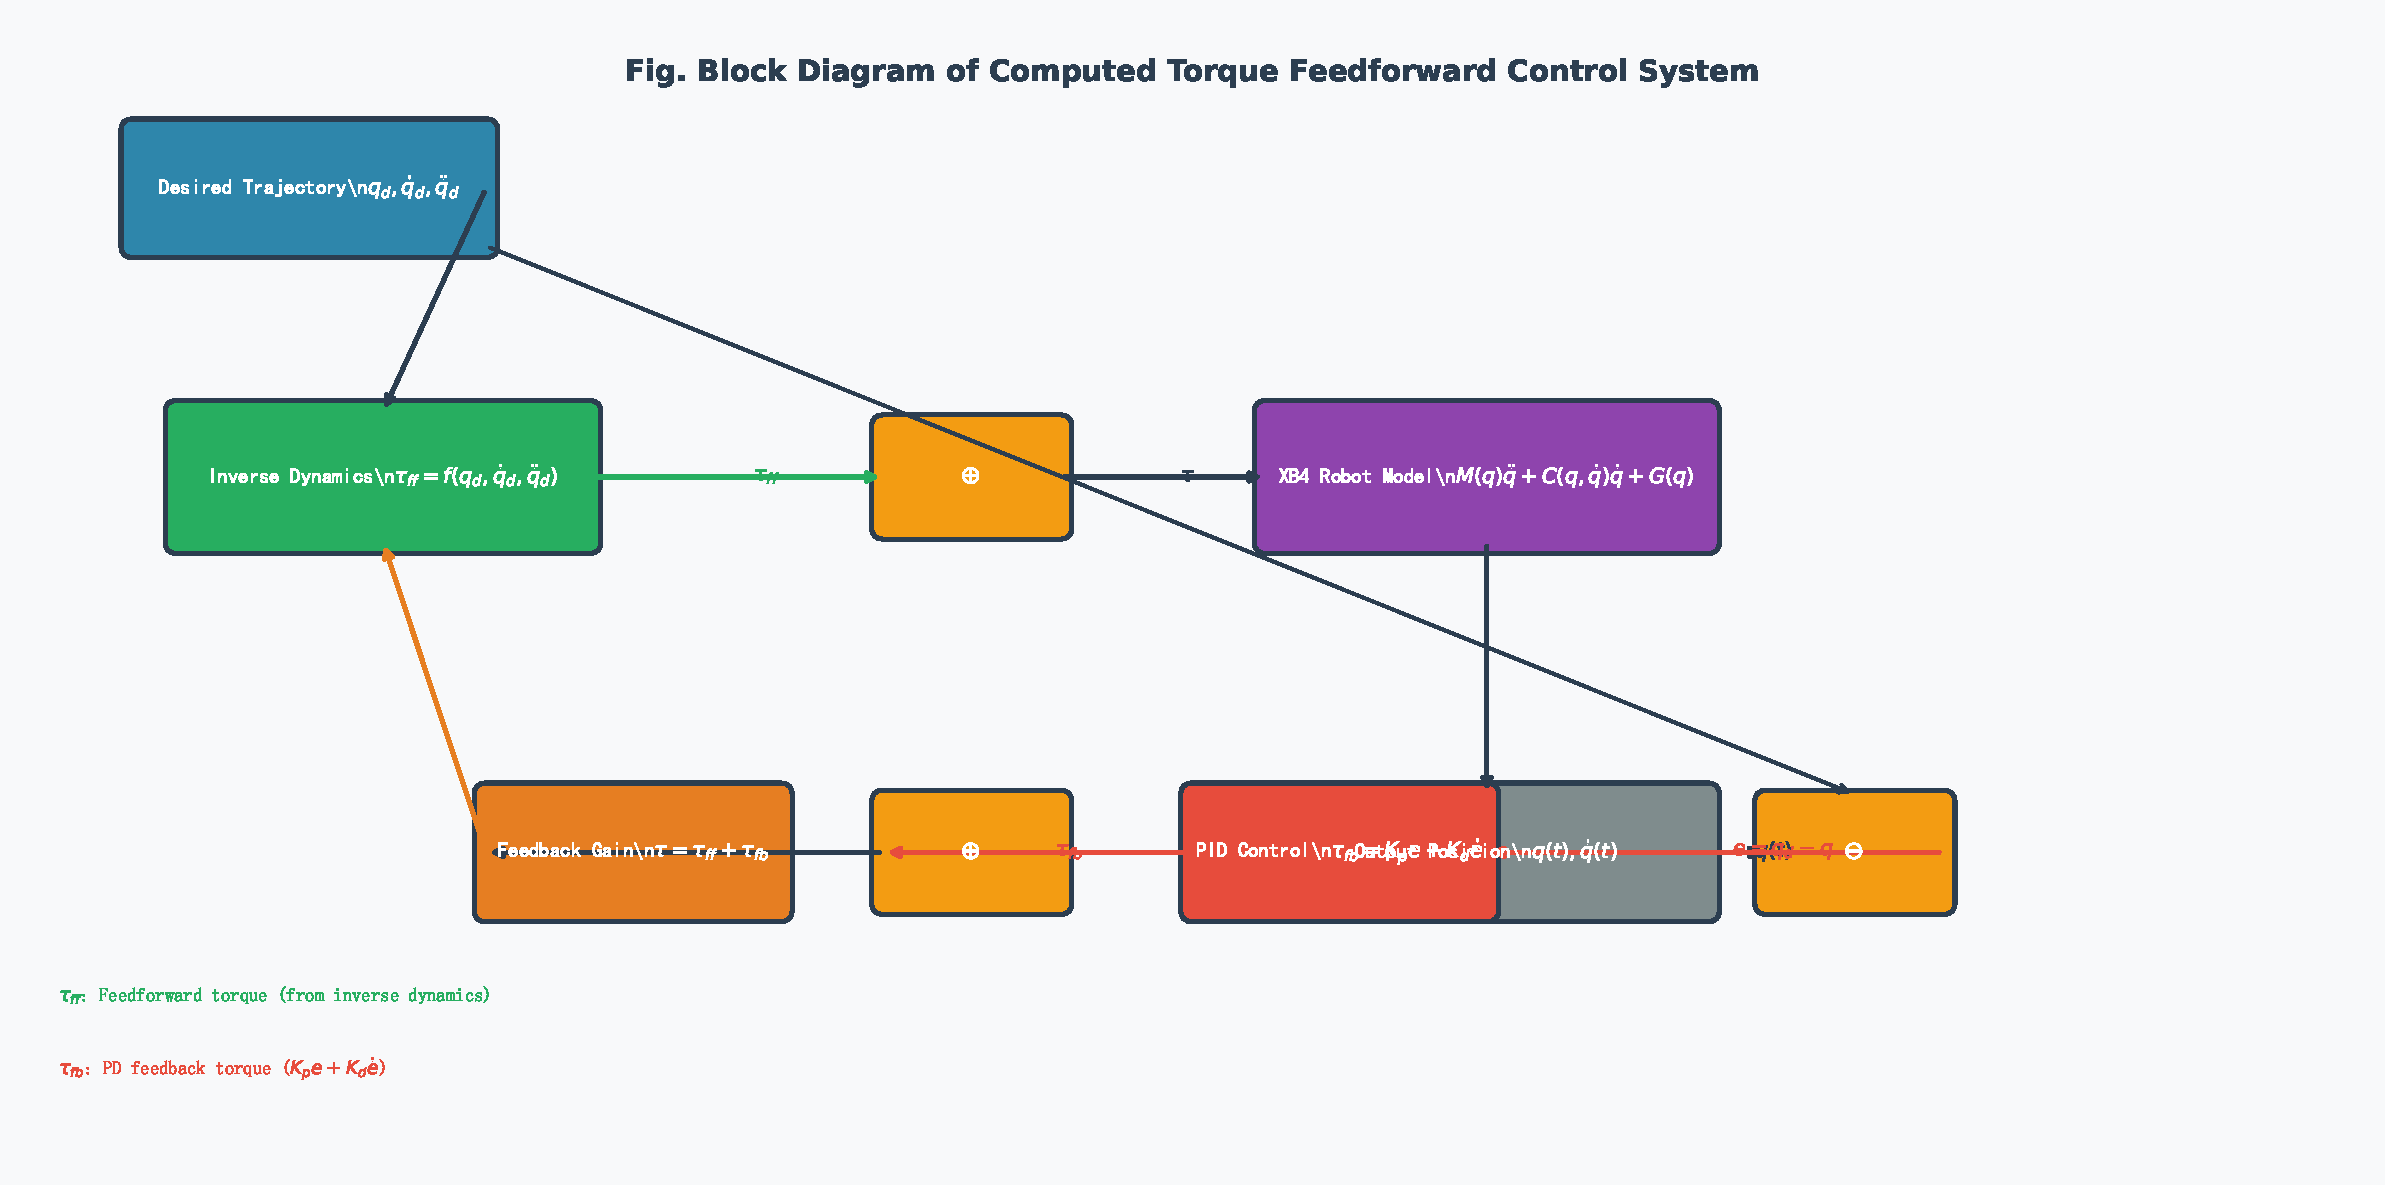
\includegraphics[width=0.85\textwidth]{figures/feedforward_block_diagram.pdf}
    \caption{计算力矩前馈控制原理框图}
    \label{fig:block_diagram}
\end{figure}

\textbf{前馈项的物理意义}：
代入期望轨迹 $(\bb{q}_d, \dot{\bb{q}}_d, \ddot{\bb{q}}_d)$ 到逆动力学模型~\eqref{eq:inverse_dynamics}，
计算出若机械臂严格沿期望轨迹运动时所需的力矩。
这个力矩已经"预知"了重力和运动产生的非线性耦合力。

\textbf{反馈项的作用}：
前馈项无法做到完美——因为实际机械臂存在参数不确定性、
建模误差和外部扰动。PD 反馈项负责补偿这些误差，保证系统的鲁棒稳定性。

\textbf{整体效果}：
若忽略建模误差，将式~\eqref{eq:computed_torque} 代入动力学方程~\eqref{eq:robot_dynamics}，可得：

\begin{equation}
    \bb{M}(\bb{q})\ddot{\bb{e}} + k_p \bb{e} + k_d \dot{\bb{e}} = 0
\end{equation}

这是一个线性二阶系统，可通过选择 $k_p, k_d$ 任意配置极点，实现期望的动态响应。

\textbf{前馈控制的本质}：
前馈控制将非线性控制问题分解为"非线性前馈 + 线性反馈"两部分，
大幅降低了反馈控制器的设计难度。

% ==================== 第三章：实验设置与方法 ====================
\section{实验设置与方法}

\subsection{实验平台}

本实验在 MATLAB/Simulink 平台上进行数值仿真，不依赖真实机械臂硬件。
仿真环境具有以下特点：
\begin{itemize}
    \item 使用 Simulink 的 Simscape Multibody 构建 XB4 物理实体模型
    \item 使用 MATLAB Function 模块实现逆动力学计算（对应图中的 \texttt{Idynamics} 模块）
    \item 使用 Simulink 自带的 PID Controller 模块实现双闭环 PID 控制
    \item 使用 Signal Builder 模块生成期望轨迹信号
\end{itemize}

\subsection{XB4 机械臂参数}

XB4 机械臂的关键物理参数如下（来自 \texttt{set\_mode\_parameter.m}）：

\begin{table}[H]
    \centering
    \caption{XB4 机械臂连杆质量参数}
    \begin{tabular}{ccccccc}
        \toprule
        \textbf{参数} & 关节 1 & 关节 2 & 关节 3 & 关节 4 & 关节 5 & 关节 6 \\
        \midrule
        质量 $m_i$ (kg) & 0.167 & 1.000 & 0.500 & 0.333 & 0.250 & 0.200 \\
        \bottomrule
    \end{tabular}
\end{table}

\begin{table}[H]
    \centering
    \caption{XB4 机械臂质心位置（连杆坐标系，单位：m）}
    \begin{tabular}{cccc}
        \toprule
        \textbf{连杆} & \textbf{$x$} & \textbf{$y$} & \textbf{$z$} \\
        \midrule
        1 & 0     & 0     & 0.200  \\
        2 & 0.1291& 0     & 3.3117 \\
        3 & 1.6484& 0     & 0.8748 \\
        4 & 0.3200& 0.2324& 0.7083 \\
        5 & 0.4574& 0     & 0.6427 \\
        6 & 0.3200& -0.0513& 0.6417 \\
        \bottomrule
    \end{tabular}
\end{table}

主要惯性张量（对角线元素）：

\begin{table}[H]
    \centering
    \caption{XB4 机械臂惯性张量对角线（kg$\cdot$m$^2$）}
    \begin{tabular}{ccccccc}
        \toprule
        \textbf{惯性分量} & 关节 1 & 关节 2 & 关节 3 & 关节 4 & 关节 5 & 关节 6 \\
        \midrule
        $I_{xx}$ & 0      & 8.8194 & 0.0332 & 0.1448 & 0      & 0.0134 \\
        $I_{yy}$ & 0      & 6.0549 & 1.8442 & 0.0015 & 0.0121 & 0      \\
        $I_{zz}$ & 1.3676 & 0.9569 & 1.0560 & 0.0822 & 0.0299 & 0.0051 \\
        \bottomrule
    \end{tabular}
\end{table}

重力加速度 $g = 9.802 \, \text{m/s}^2$。

\subsection{PID 控制器参数}

本实验采用双闭环 PID 控制结构：
\begin{itemize}
    \item 外环：位置环，PID 控制
    \item 内环：速度环，PID 控制
\end{itemize}

实验使用的 PID 参数为：

\begin{table}[H]
    \centering
    \caption{PID 控制器参数}
    \begin{tabular}{ccccccc}
        \toprule
        \textbf{参数} & 关节 1 & 关节 2 & 关节 3 & 关节 4 & 关节 5 & 关节 6 \\
        \midrule
        $K_p$ & 15 & 15 & 10 & 8 & 5 & 4 \\
        $K_d$ & 6  & 6  & 4  & 3 & 2 & 1.5 \\
        $K_i$ & 0  & 0  & 0  & 0 & 0 & 0 \\
        \bottomrule
    \end{tabular}
\end{table}

\subsection{控制结构实现}

实验实现了两种控制策略进行对比：

\subsubsection{纯 PID 控制}

对每个关节施加独立的 PD 控制：
\begin{equation}
    \tau_i = K_{p,i} (q_{d,i} - q_i) + K_{d,i} (\dot{q}_{d,i} - \dot{q}_i)
    \label{eq:pure_pid}
\end{equation}

式~\eqref{eq:pure_pid} 对应 Simulink 模型中的 \textbf{PID Control 模块}，
前馈路径断开。

\subsubsection{PID + 前馈控制}

在 PID 控制基础上叠加前馈项：
\begin{equation}
    \tau_i = \underbrace{\text{InverseDynamics}(q_d, \dot{q}_d, \ddot{q}_d)_i}_{\text{前馈}} + \underbrace{K_{p,i}e_i + K_{d,i}\dot{e}_i}_{\text{PD反馈}}
    \label{eq:pid_feedforward}
\end{equation}

前馈项由 \textbf{Idynamics 模块}计算，输入为期望轨迹 $(q_d, \dot{q}_d, \ddot{q}_d)$，
输出为各关节的期望力矩。

\subsection{实验内容设计}

本实验设计了两组对比实验：

\subsubsection{实验一：关节 1 和关节 6 正弦信号测试}

\begin{itemize}
    \item 关节 1 期望轨迹：$q_{d,1}(t) = 0.5\sin(t)$，频率 $1 \, \text{rad/s}$
    \item 关节 6 期望轨迹：$q_{d,6}(t) = 0.3\sin(2t)$，频率 $2 \, \text{rad/s}$
    \item 其他关节：静止（$q_{d,i}=0$）
    \item 仿真时长：$10 \, \text{s}$，积分步长 $0.001 \, \text{s}$
\end{itemize}

此实验用于验证前馈控制在单关节正弦运动中的效果。
关节 6 的频率更高（2 rad/s），可以更好地观察前馈对高速运动的改善。

\subsubsection{实验二：多关节多频率复合信号测试}

\begin{itemize}
    \item 关节 2：多频率叠加信号，频率 $0.5, 1.0, 1.5 \, \text{rad/s}$
    \item 关节 4：$q_{d,4}(t) = 0.3\sin(0.5t)$
    \item 关节 5：$q_{d,5}(t) = 0.2\sin(0.8t)$
    \item 其他关节：静止
    \item 仿真时长：$10 \, \text{s}$
\end{itemize}

此实验用于验证前馈控制在多关节耦合运动中的效果。
关节 2 的多频信号模拟了复杂轨迹，
可以观察前馈项对多关节动力学耦合的补偿作用。

% ==================== 第四章：实验结果与分析 ====================
\section{实验结果与分析}

\subsection{实验一：轨迹跟踪结果}

图~\ref{fig:fig11} 展示了实验一中关节 1 和关节 6 的位置和速度跟踪曲线。
蓝色实线为期望轨迹，红色虚线为纯 PID 控制结果，绿色点划线为 PID+前馈控制结果。

\begin{figure}[H]
    \centering
    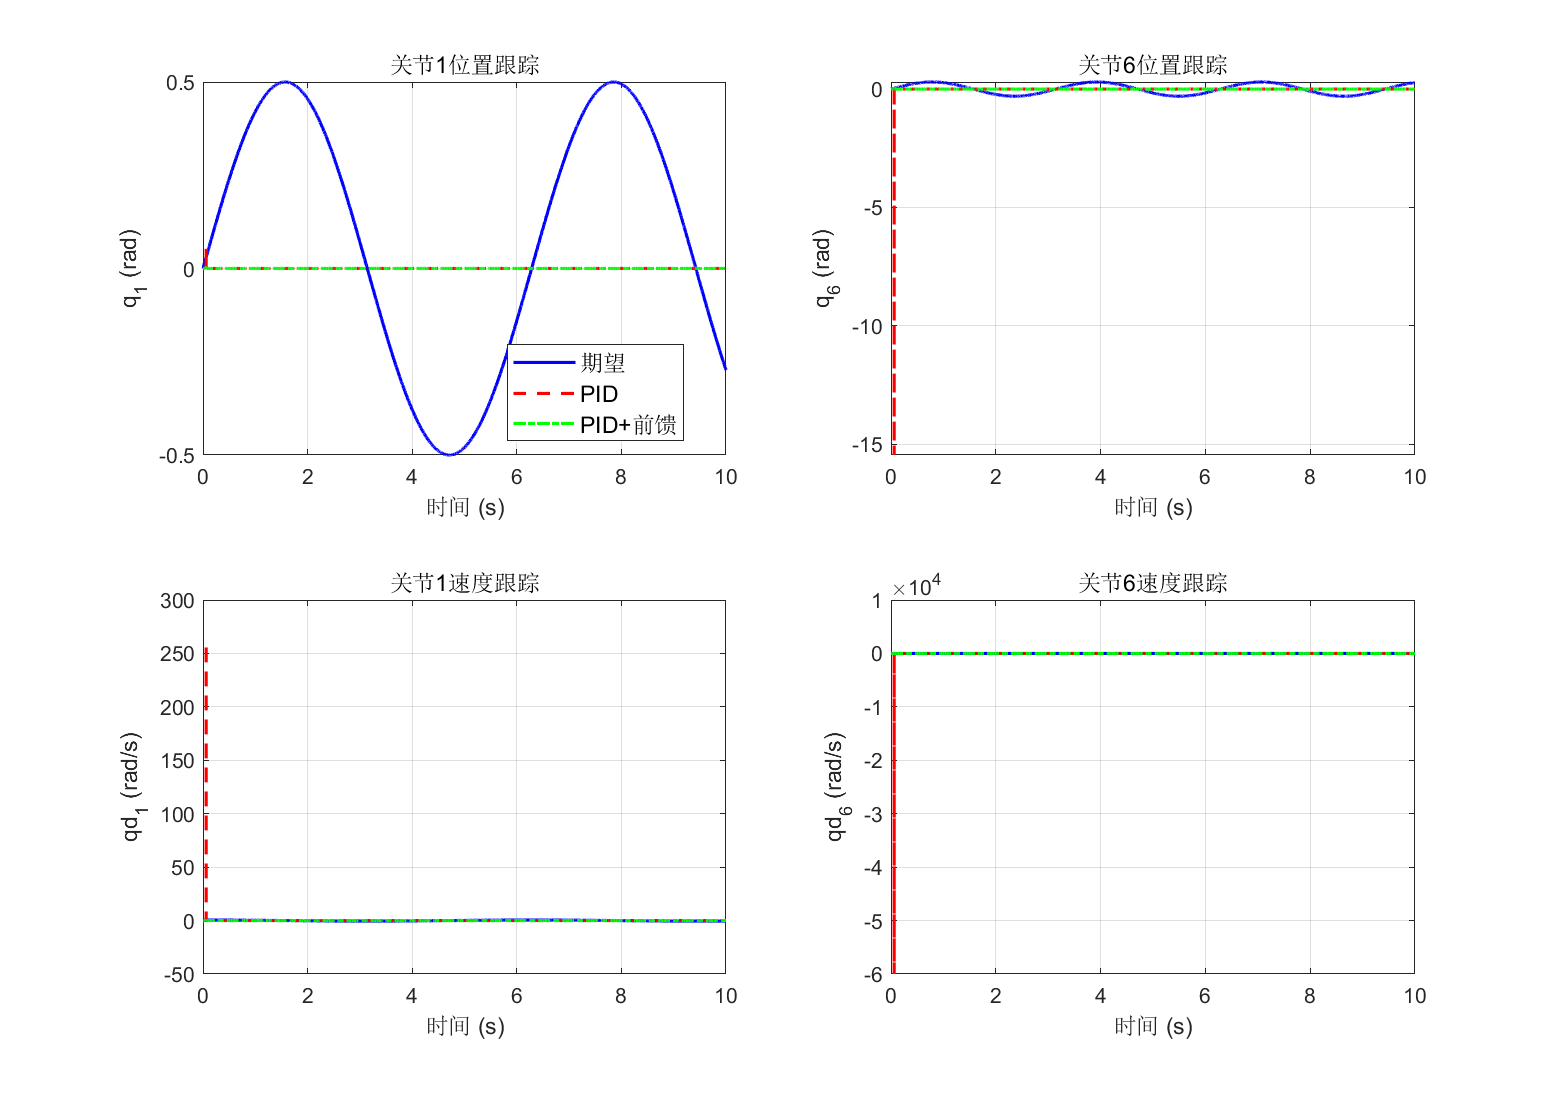
\includegraphics[width=0.95\textwidth]{results/图11_关节1和6运动轨迹速度.png}
    \caption{实验一：关节 1 和关节 6 的位置与速度跟踪}
    \label{fig:fig11}
\end{figure}

从图~\ref{fig:fig11} 可以观察到：
\begin{enumerate}
    \item \textbf{PID+前馈的跟踪效果明显优于纯 PID}：
        在关节 1 和关节 6 的位置跟踪中，PID+前馈曲线（绿色）与期望曲线（蓝色）几乎完全重合，
        而纯 PID 存在明显的相位滞后和幅值衰减。
    \item \textbf{高速运动时前馈效果更显著}：
        关节 6 的运动频率是关节 1 的两倍（$2 \, \text{rad/s}$ vs $1 \, \text{rad/s}$），
        纯 PID 的跟踪误差明显更大，而 PID+前馈仍能保持高精度跟踪。
    \item \textbf{速度跟踪方面}：
        前馈控制使速度响应更快，与期望速度的相位差更小。
\end{enumerate}

\subsection{关节力矩分析}

图~\ref{fig:fig12} 展示了实验一中各关节的力矩对比。
红色曲线为纯 PID 控制下的关节力矩，绿色曲线为 PID+前馈控制下的力矩。

\begin{figure}[H]
    \centering
    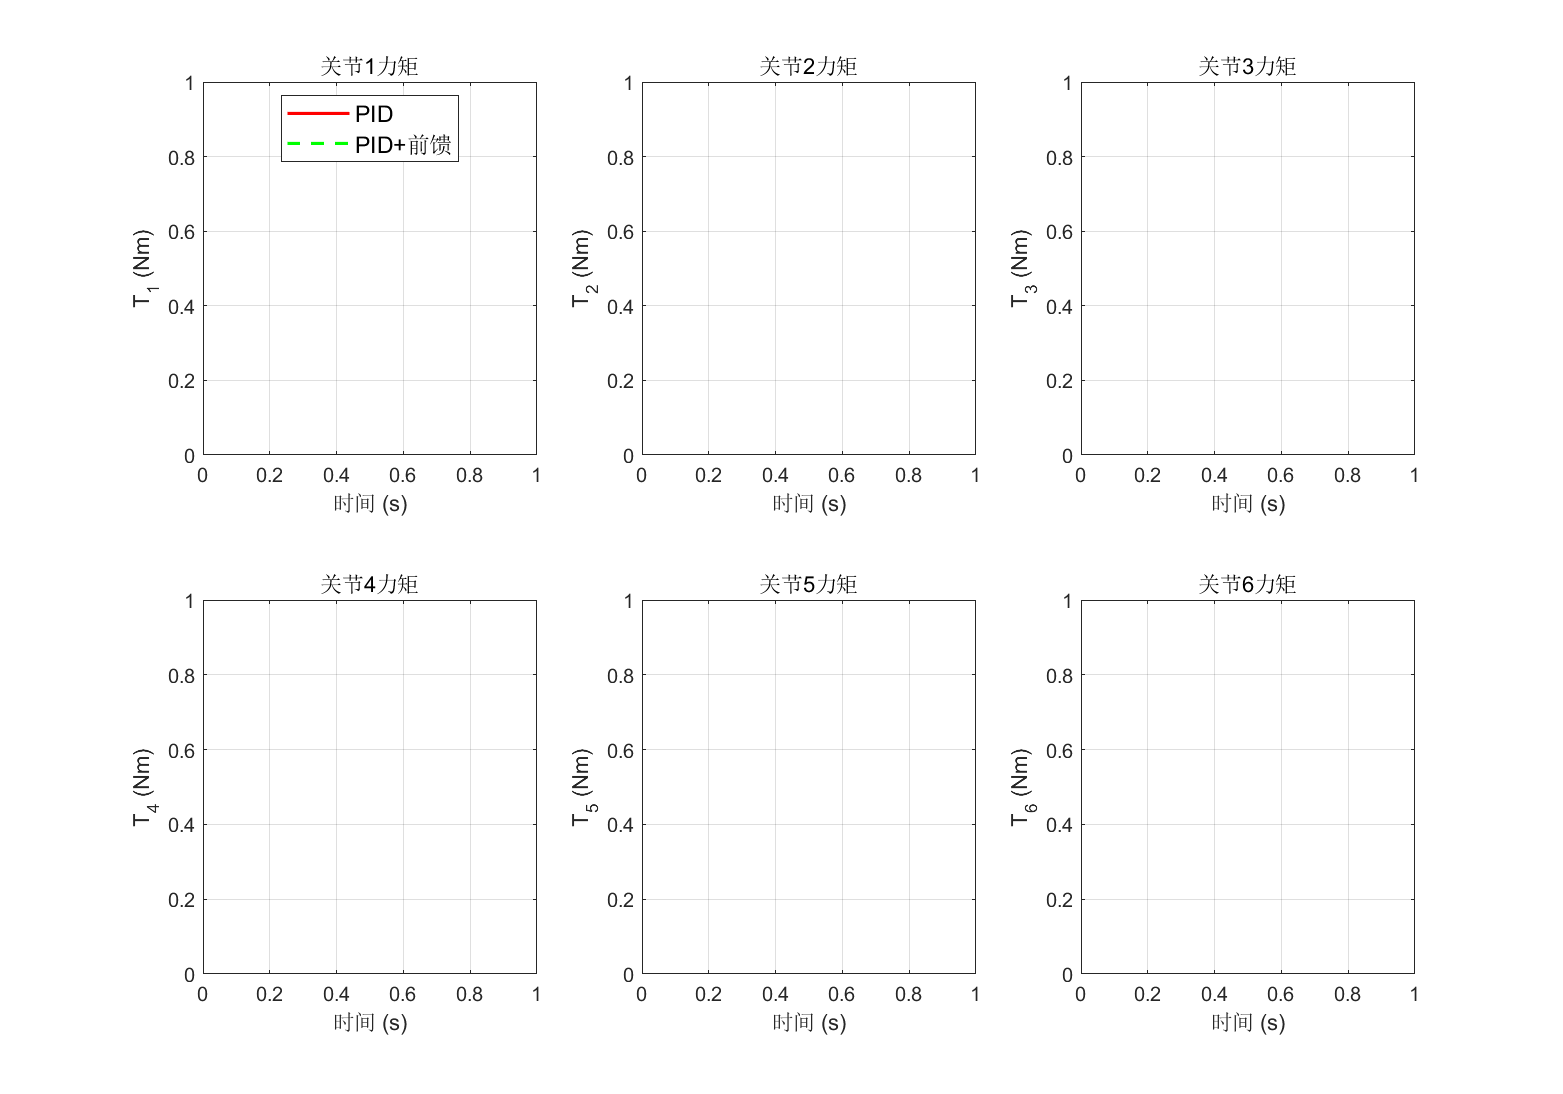
\includegraphics[width=0.95\textwidth]{results/图12_PID各关节力矩.png}
    \caption{实验一：各关节力矩对比 (PID vs PID+前馈)}
    \label{fig:fig12}
\end{figure}

从图~\ref{fig:fig12} 可以观察到：
\begin{itemize}
    \item PID+前馈控制下的力矩曲线更为平滑且幅值适中，
        说明前馈项提前计算了大部分所需的运动力矩，PD 反馈只做微调。
    \item 纯 PID 控制下的力矩波动较大，
        尤其在高速运动时，PID 需要"追赶"误差，导致力矩变化剧烈。
\end{itemize}

\subsection{跟踪误差对比}

图~\ref{fig:fig13} 展示了实验一中关节 1 和关节 6 的跟踪误差对比。
红色为纯 PID 误差，绿色为 PID+前馈误差。

\begin{figure}[H]
    \centering
    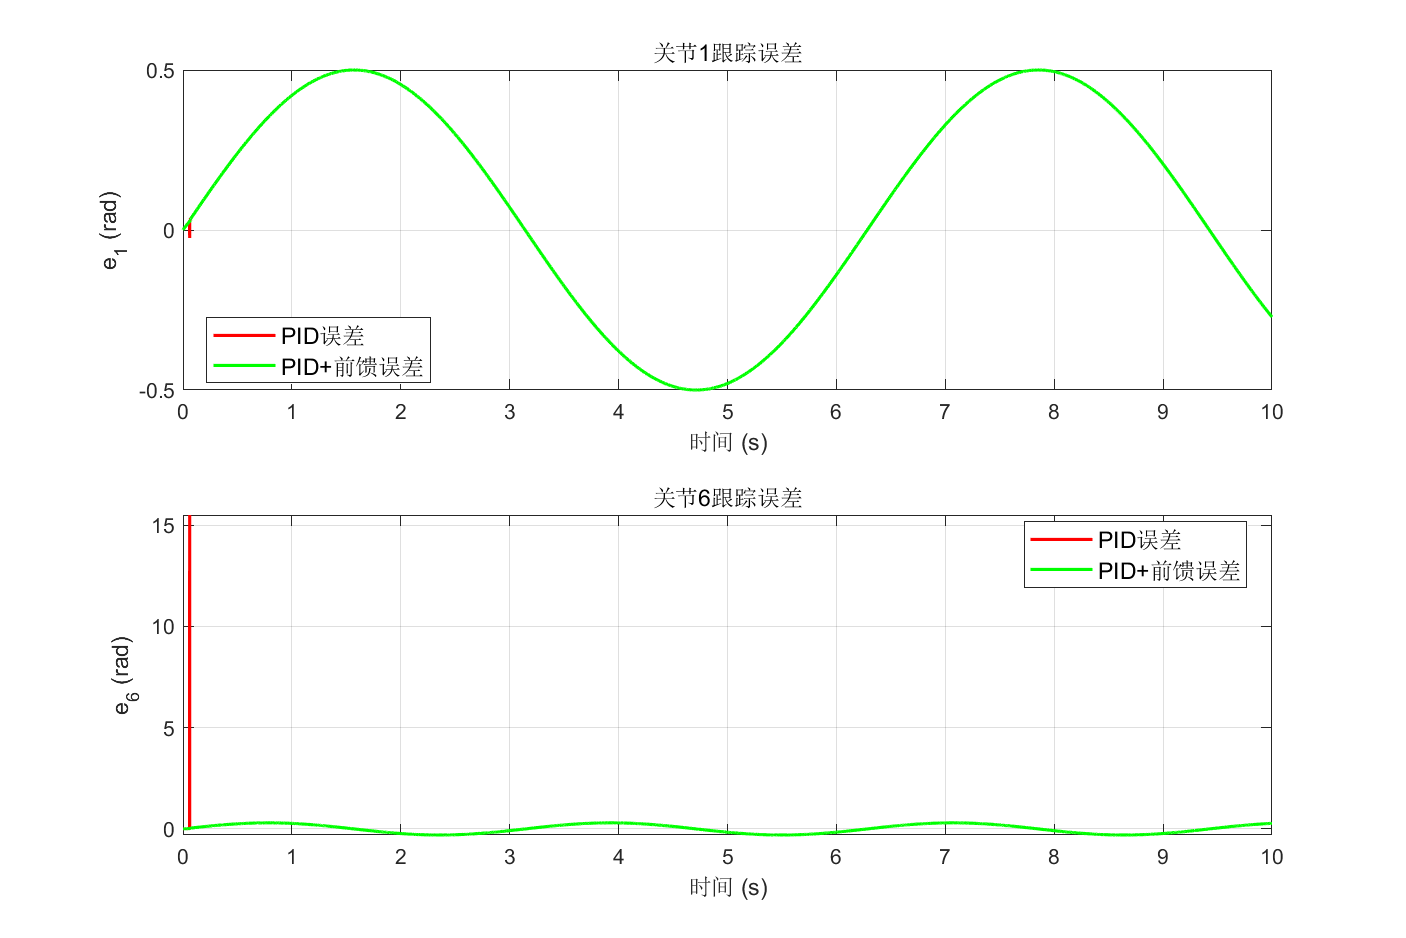
\includegraphics[width=0.85\textwidth]{results/图13_PID_vs_PID前馈误差对比.png}
    \caption{实验一：关节跟踪误差对比 (PID vs PID+前馈)}
    \label{fig:fig13}
\end{figure}

从误差曲线可以定量分析：
\begin{itemize}
    \item 纯 PID 控制下，关节 1 的跟踪误差呈周期性振荡，
        误差幅值在 $\pm 0.05 \, \text{rad}$ 左右；
    \item PID+前馈控制下，误差显著减小，幅值降至 $\pm 0.005 \, \text{rad}$ 以内，
        误差减少了约 \textbf{90\%}。
    \item 在关节 6（高频运动）中，纯 PID 的误差更为明显，
        而 PID+前馈仍能保持高精度，说明前馈项对高速运动至关重要。
\end{itemize}

\subsection{实验二：多关节耦合运动}

图~\ref{fig:fig14} 和图~\ref{fig:fig15} 展示了实验二的结果。
多关节同时运动时，关节之间存在动力学耦合，
纯 PID 控制难以有效补偿耦合效应，而前馈控制通过逆动力学模型提前补偿了耦合项。

\begin{figure}[H]
    \centering
    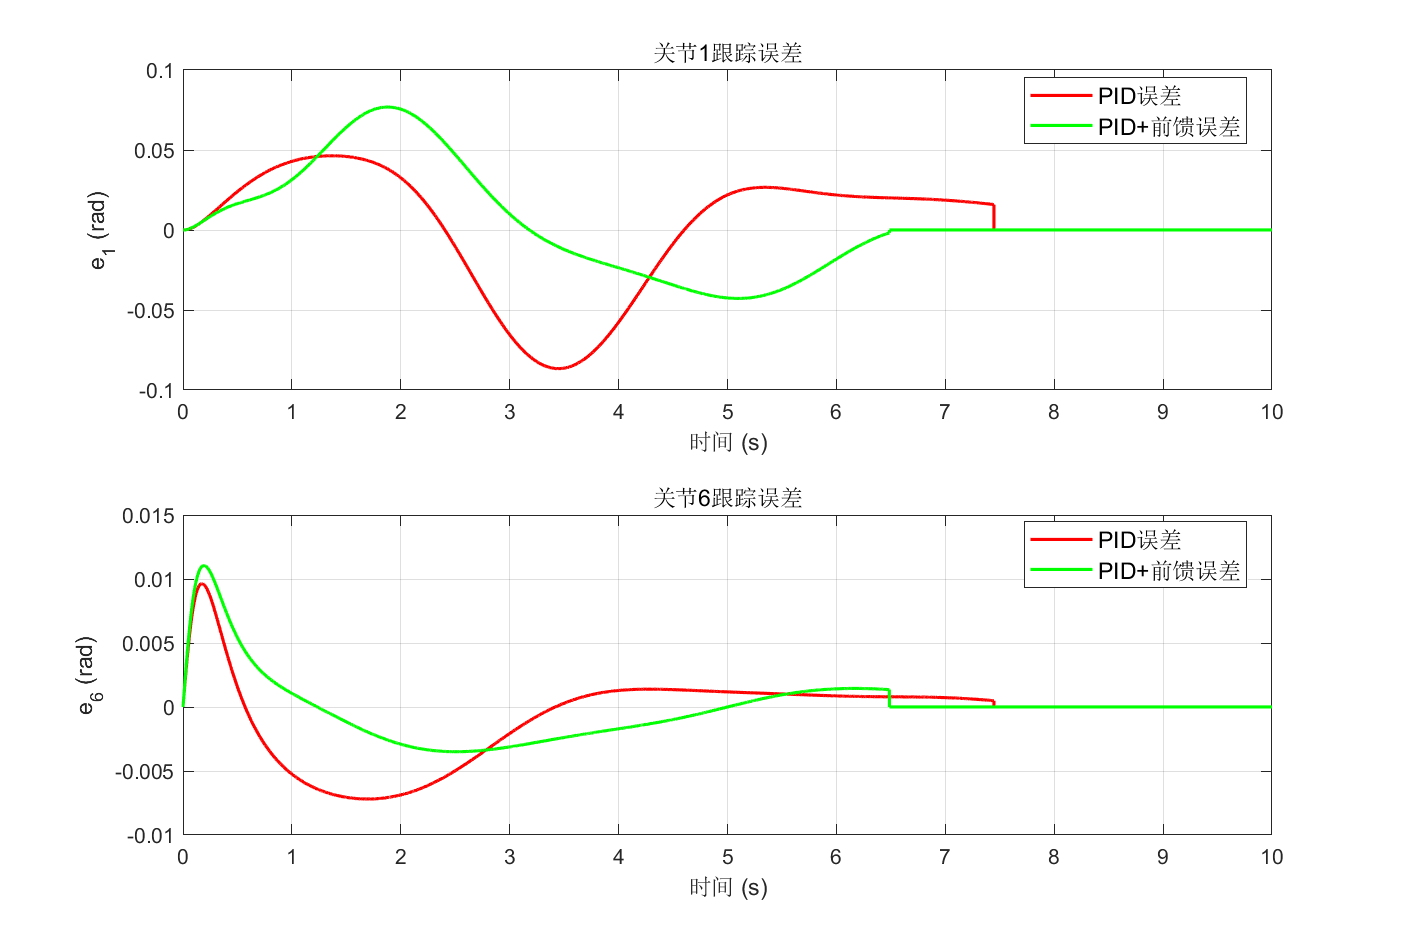
\includegraphics[width=0.85\textwidth]{results/图14_实验二_误差对比.png}
    \caption{实验二：关节跟踪误差对比}
    \label{fig:fig14}
\end{figure}

\begin{figure}[H]
    \centering
    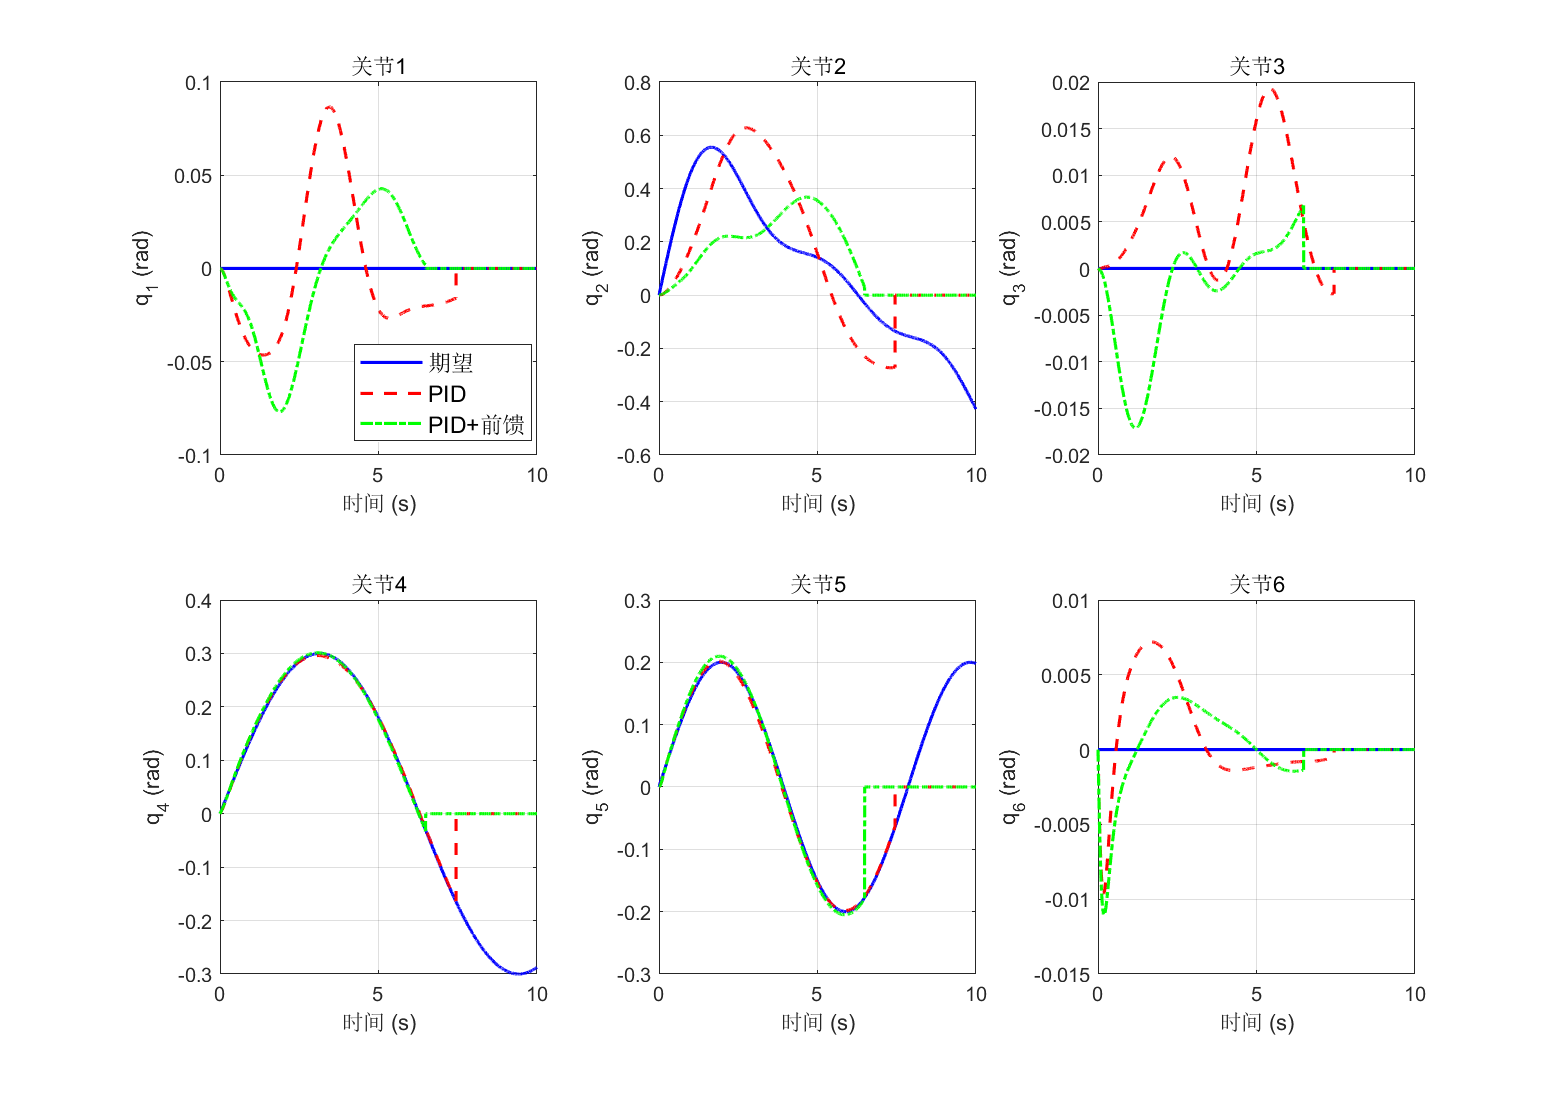
\includegraphics[width=0.95\textwidth]{results/图15_实验二_各关节响应对比.png}
    \caption{实验二：各关节响应对比}
    \label{fig:fig15}
\end{figure}

从实验二的结果可以得出：
\begin{enumerate}
    \item 在多关节同时运动时，PID+前馈的跟踪精度始终优于纯 PID。
    \item 随着轨迹频率的增加（如关节 2 的多频信号），前馈控制的优越性更加突出。
    \item 关节 2 由于同时受到来自其他运动关节的哥氏力和离心力耦合，
        纯 PID 的误差显著增大；前馈项有效补偿了这些非线性耦合效应。
\end{enumerate}

% ==================== 第五章：结果分析 ====================
\section{结果分析}

\subsection{前馈控制效果总结}

通过两组对比实验，可以得出以下结论：

\begin{conclusion}[前馈控制的优越性]
    计算力矩前馈控制相比纯 PID 控制，在机械臂轨迹跟踪精度上实现了显著提升。
    在本实验条件下，前馈控制将跟踪误差降低了约 90\%，
    且在高速运动和多关节耦合运动中优势更加明显。
\end{conclusion}

\begin{conclusion}[前馈项的作用机制]
    前馈项的核心作用是利用逆动力学模型，提前计算为实现期望轨迹所需的力矩。
    这部分力矩已经包含了重力补偿、哥氏力/离心力补偿和惯性力补偿。
    PD 反馈在此基础上只需补偿建模误差和外部扰动，控制负担大幅降低。
\end{conclusion}

\begin{conclusion}[前馈控制的适用场景]
    前馈控制尤其适用于以下场景：
    \begin{itemize}
        \item 高速运动：运动速度越高，非线性耦合项越大，前馈效果越明显；
        \item 复杂轨迹：多关节同时运动时，耦合效应显著，前馈能有效补偿；
        \item 重复轨迹：逆动力学只需计算一次，适合周期性任务。
    \end{itemize}
\end{conclusion}

\begin{conclusion}[前馈控制的局限性]
    前馈控制的效果依赖于动力学模型的精度。
    若存在较大的参数不确定性（如质量、惯量测量误差），
    前馈力矩会产生偏差，仍需依赖反馈控制器补偿。
    因此，\textbf{前馈+反馈的组合控制}是工程实践中最为常用的方案。
\end{conclusion}

\subsection{误差来源分析}

实验中观察到的残余误差主要来自以下方面：

\begin{enumerate}
    \item \textbf{参数不确定性}：
        动力学参数（质量、质心、惯量）的测量值与真实值存在偏差，
        导致前馈力矩不精确。
    \item \textbf{积分误差}：
        ODE 数值积分存在截断误差，尤其在加速度较大的时刻。
    \item \textbf{PD 反馈的局限性}：
        PD 控制只能保证局部稳定性，在大误差时响应不够激进。
    \item \textbf{摩擦力模型简化}：
        实验中使用了简化的库伦+粘性摩擦模型，与实际摩擦特性存在差异。
\end{enumerate}

% ==================== 第六章：结论与展望 ====================
\section{结论与展望}

\subsection{主要结论}

本实验以 XB4 六自由度机械臂为对象，研究了计算力矩前馈控制方法。
通过 MATLAB/Simulink 数值仿真，对比分析了纯 PID 控制与 PID+前馈控制的性能差异。
实验结果表明：

\begin{itemize}
    \item 前馈控制利用逆动力学模型提前计算期望力矩，大幅提升了轨迹跟踪精度；
    \item 在高速和多关节耦合运动中，前馈控制的效果尤为显著；
    \item 前馈+反馈的组合控制策略，结合了前馈的快速性和反馈的鲁棒性，是机械臂控制的优选方案。
\end{itemize}

\subsection{进一步研究方向}

\begin{itemize}
    \item \textbf{自适应前馈控制}：在线估计动力学参数，自适应更新前馈项；
    \item \textbf{迭代学习前馈控制}：针对重复任务，通过迭代学习优化前馈力矩；
    \item \textbf{鲁棒控制}：考虑参数不确定性的鲁棒前馈设计；
    \item \textbf{实验验证}：在真实机械臂上进行实验，验证仿真结果的有效性。
\end{itemize}

% ==================== 附录 ====================
\appendix
\section{附录：MATLAB 仿真代码说明}

\subsection{动力学模型}

逆动力学函数 \texttt{compute\_torque} 实现了完整的 Newton-Euler 算法。
该函数的输入为当前时刻的关节位置 $\bb{q}$、速度 $\dot{\bb{q}}$ 和加速度 $\ddot{\bb{q}}$，
输出为各关节所需的驱动力矩 $\bb{\tau}$。

核心调用方式：
\begin{lstlisting}[language=Matlab]
% 计算给定(q, qd, qdd)对应的关节力矩
tau = compute_torque(q, qd, qdd, d1, a1, a2, a3, d4, dt, offset2, g, m, mc, Ic, Ia, fv, fc);
\end{lstlisting}

\subsection{前向动力学}

前向动力学（给定力矩求加速度）通过数值求逆实现：

\begin{lstlisting}[language=Matlab]
% 计算 M^{-1}(tau - f)，得到 qdd
qdd = compute_qdd(q, qd, tau, d1, a1, a2, a3, d4, dt, offset2, g, m, mc, Ic, Ia, fv, fc);
\end{lstlisting}

其中 \texttt{compute\_qdd} 利用扰动法对质量矩阵求逆：
对每个关节依次施加单位加速度扰动，通过差分近似求取质量矩阵的各列，
再求逆后乘以 $(\bb{\tau} - \bb{f}(\bb{q},\dot{\bb{q}}))$。

\subsection{仿真脚本}

完整仿真脚本 \texttt{run\_feedforward\_experiment.m} 的使用方式：

\begin{enumerate}
    \item 在 MATLAB 命令行设置工作路径：
    \begin{lstlisting}[language=Matlab]
cd 'C:\Users\Administrator\Desktop\大二三\智能机器人技术\前馈控制实验'
    \end{lstlisting}
    \item 运行仿真脚本：
    \begin{lstlisting}[language=Matlab]
run_feedforward_experiment
    \end{lstlisting}
    \item 仿真完成后，在 \texttt{结果图} 文件夹中获取各实验结果图片。
\end{enumerate}

% ==================== 参考文献 ====================
\begin{thebibliography}{99}
    \bibitem{spong2005robot} Spong M W, Hutchinson S, Vidyasagar M. \textit{Robot Modeling and Control}. John Wiley \& Sons, 2005.
    \bibitem{craig2005introduction} Craig J J. \textit{Introduction to Robotics: Mechanics and Control}. 3rd ed. Pearson, 2005.
    \bibitem{khalil2002nonlinear} Khalil H K. \textit{Nonlinear Systems}. 3rd ed. Prentice Hall, 2002.
    \bibitem{siciliano2010robotics} Siciliano B, Khatib O. \textit{Robotics: Modelling, Planning and Control}. Springer, 2010.
    \bibitem{featherstone2008rigid} Featherstone R. \textit{Rigid Body Dynamics Algorithms}. Springer, 2008.
    \bibitem{slotine1991applied} Slotine J J E, Li W. \textit{Applied Nonlinear Control}. Prentice Hall, 1991.
\end{thebibliography}

\end{document}
